%% ------------------------------------------------------------------------- %%
\chapter{Evaluation}
\label{cap:experimentos}

In this chapter we present some experimental evaluations of the proposed extensions along with the original method in four widely known datasets: SFA, Pratheepan, HGR, and Compaq. In addition, a brief definition of the evaluation metrics used is shown for the sake of clarity. We also provide some results of the supplementary neighborhood adaptation that we built to remove the \emph{diagonal effect} as well as to explore different neighbors techniques. Finally, we show the grid search parameters experiments results with aim of trapezoids parameters tuning. All the experiments are analyzed and discussed in each section separately.


%------------------------------------------------------
\section{Datasets}
\label{sec:datasets}
Datasets are an integral part of the field of computer vision. In the particular case of computer vision, datasets consist, primarily, of images or videos for tasks such as object detection, motion tracking, segmentation, and classification. In general, they are constructed with tens, hundreds, or even thousands of images in different environments, distinct illumination conditions, various quality and resolution, and many other aspects.

We gathered four widely known datasets, SFA, Pratheepan, HGR, and Compaq, which will be briefly introduced in next sections, to be used in our experiments. Together, they sum up 7,423 images in different size and resolution, and more than 1.5 billion pixels tested in all the experiments, counting only the original images.


%------------------------------------------------------
\subsection{UCI}
\label{sec:datasets_uci}
Named UCI in this work, this dataset was proposed by~\citet{uci-skin-dataset:12} and obtained from the machine learning repository of the University of California in Irvine~\citep{lichman:13}. The dataset consists of pixel samples of images of various skin and non-skin textures obtained from thousands of arbitrary faces images of different ages, gender, and races~\citep{pal-texas:04, feret:96}.

The UCI contains 245,057 samples, composed of 3 attributes that constitute the input vector $x = [x_1, x_2, x_3]$, $x \in \mathbb{R}^{d}$, where $d$ is the space dimension which represents, respectively, blue (B), green (G) and red (R) channels of the RGB color model. In addition, a fourth column determines the class to which the sample $x$ belongs, denoted by $y$, where $y \in Y$ and $Y = \{+1, -1\}$. In other words, each sample is an RGB pixel with a given label.

The Table~\ref{tbl:uci_dataset} exemplifies a short excerpt from the UCI database. It is worth mentioning that 194,198 out of the 245,057 are non-skin pixels and 50,859 pixels with different skin tones. In addition, the images that were used to extract the dataset were not made available by the authors.

\begin{table}[H]
\centering
\begin{small}
\begin{tabular}{|c|c|c|c|} \hline
\thb{B} & \thb{G} & \thb{R}  & \thb{Label}  \\ \hline
74	    & 85      & 123	     & 1     \\
207	    & 215     & 255      & 1     \\
74      & 82      & 122	     & 1     \\
202     & 211     & 255      & 1     \\
54      & 72      & 125      & 1     \\
\ldots  &\ldots   & \dots    &\ldots \\
166     & 164     & 116      & -1    \\
148     & 150     & 91       & -1    \\
29      & 26      & 5        & -1    \\
167     & 166	  & 115	     & -1    \\
180	    & 177	  & 133	     & -1    \\ \hline
\end{tabular}
\caption[Excerpt with samples from the UCI dataset]{Excerpt with samples from the UCI dataset. Each of the first three columns represents a pixel channel of the RGB color space ranging from 0 to 255. The fourth column is the label assigned to the sample, which can assume +1 if it is skin and -1, otherwise. Originally, the class representing a non-skin pixel had value 2, replaced by -1 for compliance with the experiments.}
\label{tbl:uci_dataset}
\end{small}
\end{table}

Since the data are points in the RGB space, it is possible to plot it for a better interpretation of them, as shown in the Figure~\ref{fig:dataset_uci}.

\begin{figure}[H]
    \centering
    \begin{minipage}{0.45\textwidth}
        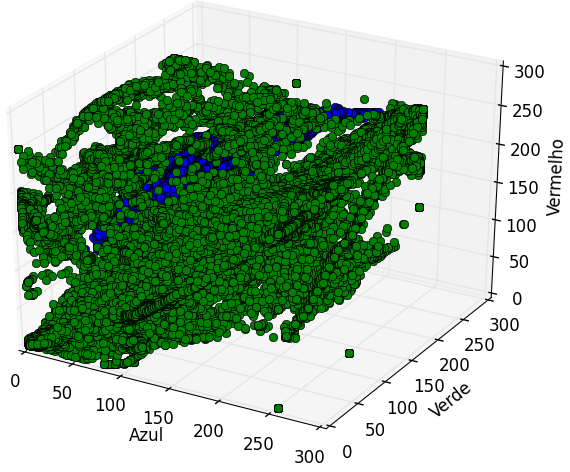
\includegraphics[width=\textwidth]{uci_skinns_plot}
    \end{minipage}
    ~ % space
    \begin{minipage}{0.45\textwidth}
        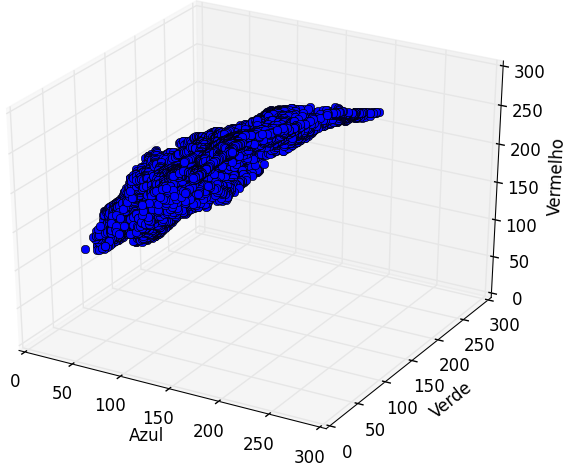
\includegraphics[width=\textwidth]{uci_skin_plot}
    \end{minipage}
    \caption[3-dimensional view of the RGB channels of the UCI dataset]{3-dimensional view of the RGB channels of the UCI dataset. The blue points are skin samples and the green ones are non-skin. On the left are all samples of the dataset; to the right only the skin samples. Source: proposed by the author.}
    \label{fig:dataset_uci}
\end{figure}


%------------------------------------------------------
\subsection{SFA}
\label{sec:datasets_sfa}
SFA, the name of the dataset proposed by~\citet{sfa-skin-dataset:13}, stands for Skin of FERET and AR Database. The SFA is a set of images of frontal faces obtained from two other color image databases: the FERET, created by~\citet{feret:96}, and the AR proposed by~\citet{ar-face-database:98}, which provided 876 and 242 images each, respectively. It is important to notice that AR images have a white background and small variations of skin color. In other words, the environment is more controlled than the images in FERET~\citep{sfa-skin-dataset:13}. Figure~\ref{fig:sfa_dataset_exemplo} shows some of the 1,118 samples available.

\citet{sfa-skin-dataset:13} also extracted different window patches of each skin and non-skin samples to facilitate future research. The samples were randomly generated considering the ground truth mask \footnote{Ground truth is the term used to denote an image whose point of interest is properly segmented and highlighted, discarding the remaining pixels giving them uniform colors.} of each image, being three samples of skin and five of non-skin. Each sample is a window of size $n \times n$, where $n$ is odd, with a central pixel, from which other sample sizes have been created, ranging from $1 \times 1$ to $35 \times 35$, as can be seen in Figure~\ref{fig:sfa_dataset_janelas}.

\begin{figure}[H]
  \centering
  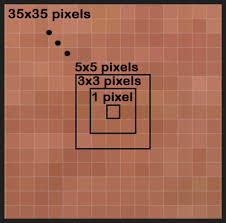
\includegraphics[width=.3\textwidth]{sfa-janelas}
  \caption[Structure of the windows that form the SFA patch samples]{Structure of the windows that form the SFA patch samples. In total, there are 3,354 skin samples and 5,590 non-skin samples for each window size. Source: \citet{sfa-skin-dataset:13}.}
  \label{fig:sfa_dataset_janelas}
\end{figure}

\begin{figure}[H]
    \centering
    \begin{subfigure}[t]{0.2\textwidth}
        \includegraphics[width=\textwidth]{sfa/ori/img4}
        \includegraphics[width=\textwidth]{sfa/gtc/img4}
        \includegraphics[width=\textwidth]{sfa/gt/img4}
    \end{subfigure}
    ~
    \begin{subfigure}[t]{0.2\textwidth}
        \includegraphics[width=\textwidth]{sfa/ori/img51}
        \includegraphics[width=\textwidth]{sfa/gtc/img51}
        \includegraphics[width=\textwidth]{sfa/gt/img51}
    \end{subfigure}
    ~
    \begin{subfigure}[t]{0.2\textwidth}
        \includegraphics[width=\textwidth]{sfa/ori/img112}
        \includegraphics[width=\textwidth]{sfa/gtc/img112}
        \includegraphics[width=\textwidth]{sfa/gt/img112}
    \end{subfigure}
    ~ % space
    \begin{subfigure}[t]{0.2\textwidth}
        \includegraphics[width=\textwidth]{sfa/ori/img14}
        \includegraphics[width=\textwidth]{sfa/gtc/img14}
        \includegraphics[width=\textwidth]{sfa/gt/img14}
    \end{subfigure}
    \caption[Examples of SFA face image database]{Examples of SFA face image database. First row are the original images and the second contain the colored ground truth with the skin color pixels annotated manually. The black color RGB = (0, 0, 0) was assigned to all pixels in the background. In the third row we have the binary ground truth images. We generated these samples based on the colored ground truth, by creating a mask, assigning (255, 255, 255) for the pixels which were not background (0, 0, 0). One can see some noise in the results, but the samples were enough for further experiments. In addition, the original images were not perfectly annotated. Therefore, some salt noise can be seen in non-skin regions. Source:~\citet{sfa-skin-dataset:13}.}
    \label{fig:sfa_dataset_exemplo}
\end{figure}

It is worth mentioning that we do not use these patches in our experiments. Once the methods tested in this work only depends on the input image itself. Therefore, we can simply ignore these sampling patches during experiments. However, one could use them to evaluate the ability of the methods in terms of false detection rate, once the patches are made available for skin and non-skin labeled images separately.


%------------------------------------------------------
\subsection{Pratheepan}
\label{sec:datasets_pratheepan}
The images in the Pratheepan dataset were downloaded randomly from Google for human skin detection research. There are 78 images of family and face captured with a range of distinct cameras using different color enhancement and under different illumination conditions~\cite{tan:12}. Figure~\ref{fig:pra_dataset_exemplo} shows some of the 78 samples available.

\begin{figure}[H]
    \centering
    \begin{subfigure}[t]{0.238\textwidth}
        \includegraphics[width=\textwidth]{pra/ori/07-c140-12family-red-rr-398h}
        \includegraphics[width=\textwidth]{pra/gt/07-c140-12family-red-rr-398h}
    \end{subfigure}
    ~
    \begin{subfigure}[t]{0.25\textwidth}
        \includegraphics[width=\textwidth]{pra/ori/3115267-My-very-large-Indian-family-2}
        \includegraphics[width=\textwidth]{pra/gt/3115267-My-very-large-Indian-family-2}
    \end{subfigure}
    ~
    \begin{subfigure}[t]{0.25\textwidth}
        \includegraphics[width=\textwidth]{pra/ori/buck_family}
        \includegraphics[width=\textwidth]{pra/gt/buck_family}
    \end{subfigure}
    ~
    \begin{subfigure}[t]{0.141\textwidth}
        \includegraphics[width=\textwidth]{pra/ori/chenhao0017me9}
        \includegraphics[width=\textwidth]{pra/gt/chenhao0017me9}
    \end{subfigure}
    \caption[Examples of Pratheepan skin dataset]{Examples of Pratheepan skin dataset. At the top row is the original image, and at the bottom row the ground truth with the skin color pixels annotated. Here, the ground truth are binary images, where the black color RGB = (0, 0, 0) was assigned to all pixels in the background. Source:~\citet{tan:12}.}
    \label{fig:pra_dataset_exemplo}
\end{figure}


%------------------------------------------------------
\subsection{HGR}
\label{sec:datasets_hgr}
The database for Hand Gesture Recognition (HGR) contains the gestures from Polish and American Sign Language. There are 1,558 images acquired in different conditions of background, dimensions and lightening. In addition to original and ground truth binary skin mask images, it includes hand feature points location in separate files. Figure~\ref{fig:hgr_dataset_exemplo} shows some of the 1,558 samples available \citep{kawulok:14, nalepa:14, grzejszczak:16}.

The images within it were acquired in three different series. A set of 899 was captured in uncontrolled background and lighting. A small set of 85 was obtained in gray (44) and uncontrolled (41) background; the lighting was uniform. The third group contains 574 images in controlled background (green tone), using uniform lighting conditions~\citep{kawulok:14, nalepa:14, grzejszczak:16}.

\begin{figure}[H]
    \centering
    \begin{subfigure}[t]{0.3\textwidth}
        \includegraphics[width=\textwidth]{hgr/ori/D_P_hgr1_id05_2}
        \includegraphics[width=\textwidth]{hgr/gt/D_P_hgr1_id05_2}
    \end{subfigure}
    ~
    \begin{subfigure}[t]{0.275\textwidth}
        \includegraphics[width=\textwidth]{hgr/ori/N_P_hgr1_id04_5}
        \includegraphics[width=\textwidth]{hgr/gt/N_P_hgr1_id04_5}
    \end{subfigure}
    ~
    \begin{subfigure}[t]{0.337\textwidth}
        \includegraphics[width=\textwidth]{hgr/ori/V_S_hgr2A2_id03_1}
        \includegraphics[width=\textwidth]{hgr/gt/V_S_hgr2A2_id03_1}
    \end{subfigure}
    \caption[Examples of HGR skin dataset]{Examples of HGR skin dataset. At the top row is the original image and at the bottom row the ground truth with the skin color pixels annotated. Differently from Pratheepan and SFA, the ground truth is also binary images, but the black color RGB = (0, 0, 0) was assigned to all pixels when they represent skin patches -- and we take this in consideration during experiments. Source:~\citet{kawulok:14, nalepa:14, grzejszczak:16}.}
    \label{fig:hgr_dataset_exemplo}
\end{figure}


%------------------------------------------------------
\subsection{Compaq}
\label{sec:datasets_compaq}
Compaq can be considered as the first large skin dataset and, probably is the most used for skin detection classifiers. It consists of 13,635 images crawled from the internet, which 4,670 contain skin regions and another subset of 8,965 images not containing any skin. The ground truth images are poorly annotated on the basis of an automatic software tool~\citep{mahmoodi:16}.

It is worth mentioning that this database is no longer available and we had obtained a copy of it by contacting the authors. We also had to fix some few images due lack of ground truth or files corrupted. The final amount of images with skin used in the experiments is 4,669. Figure~\ref{fig:compaq_dataset_example} shows some of the 4,669 images with skin samples available used in the experiments~\citep{jones:02}.

\begin{figure}[H]
    \centering
    \begin{subfigure}[t]{0.269\textwidth}
        \includegraphics[width=\textwidth]{cpq/ori/318196}
        \includegraphics[width=\textwidth]{cpq/gt/318196}
    \end{subfigure}
    ~
    \begin{subfigure}[t]{0.214\textwidth}
        \includegraphics[width=\textwidth]{cpq/ori/795505}
        \includegraphics[width=\textwidth]{cpq/gt/795505}
    \end{subfigure}
    ~
    \begin{subfigure}[t]{0.132\textwidth}
        \includegraphics[width=\textwidth]{cpq/ori/1923132}
        \includegraphics[width=\textwidth]{cpq/gt/1923132}
    \end{subfigure}
    ~
    \begin{subfigure}[t]{0.14\textwidth}
        \includegraphics[width=\textwidth]{cpq/ori/2747136}
        \includegraphics[width=\textwidth]{cpq/gt/2747136}
    \end{subfigure}
    ~
    \begin{subfigure}[t]{0.12\textwidth}
        \includegraphics[width=\textwidth]{cpq/ori/3003632}
        \includegraphics[width=\textwidth]{cpq/gt/3003632}
    \end{subfigure}
    \caption[Examples of Compaq skin/non-skin dataset]{Examples of Compaq skin/non-skin dataset. At the top row is the original image, and at the bottom the ground truth with the skin color pixels annotated. Here, the ground truth are binary images, where the black color RGB = (0, 0, 0) was assigned to all pixels in the background. Source:~\citet{jones:02}.}
    \label{fig:compaq_dataset_example}
\end{figure}



%------------------------------------------------------
\section{Evaluation measures}
\label{sec:evaluation_measures}

\textit{Precision, Recall, Specificity} and \textit{F-measure} have been used as evaluation metrics. They are the same used in~\citet{brancati:17} to compare the performance with state-of-the-art methods. They are also widely used by the scientific community. These metrics are given by the following formulas:

\begin{equation*}
    Precision = \frac{TP}{TP + FP}
    \label{eq:precision}
\end{equation*}

\begin{equation*}
    Recall = \frac{TP}{TP + FN}
    \label{eq:recall}
\end{equation*}

\begin{equation*}
    Specificity = \frac{TN}{TN + FP}
    \label{eq:specificity}
\end{equation*}

\begin{equation*}
    F-measure = 2 \times \frac{Precision \times Recall}{Precision + Recall}
    \label{eq:fmeasure}
\end{equation*}

where TP, TN, FP, FN are, respectively, the number of true positive, true negative, false positive, and false negative pixels counted in the image, which are obtained from the confusion matrix (see Table~\ref{tab:confusion_matrix}).

\begin{table}[H]
    \centering

    \begin{tikzpicture}[
    box/.style={draw,rectangle,minimum size=2cm,text width=1.5cm,align=center}]
    \matrix (conmat) [row sep=.1cm,column sep=.1cm] {
    \node (tpos) [box,
        label=left:\( \textbf{skin} \),
        label=above:\( \textbf{skin} \),
        ] {True \\ Positive};
    &
    \node (fneg) [box,
        label=above:\textbf{non-skin}] {False \\ Negative};
    \\
    \node (fpos) [box,
        label=left:\( \textbf{non-skin} \)] {False \\ Positive};
    &
    \node (tneg) [box] {True \\ Negative};
    \\
    };
    \node [left=.05cm of conmat,text width=1.5cm,align=right] {\textbf{ground \\ truth}};
    \node [above=.05cm of conmat] {\textbf{prediction outcome}};
    \end{tikzpicture}

    \caption[Confusion matrix table used during experiments]{Confusion matrix table used to count the number of true positive, true negative, false positive, and false negative pixels in the image during experiments. These numbers are fundamental input for evaluation measures.}
    \label{tab:confusion_matrix}
\end{table}




%------------------------------------------------------
\section{UCI dataset evaluation}
\label{sec:ml_experiments}
Preliminary experiments were carried out using machine learning techniques in order to evaluate the UCI dataset, described in section~\ref{sec:datasets_uci}, once we do not have the original images used to create it. The idea is to establish a bottom line to understand if this dataset can be useful for further experiments.

The first experiment was carried out with k-Nearest Neighbors ($k$-NN) and Support Vector Machines (SVM), available in the scikit-learn package~\citep{scikit-learn:11}. The color space originally used was RGB, as cited in the description of datasets in section~\ref{sec:datasets_uci}. In both cases, the chosen cross-validation strategy was 10-fold, which is a common choice of this approach in practice~\citep{mostafa:12}. In addition, the grid search technique of scikit-learn was also used with the objective of finding the most suitable parameters for each classifier.

The grid search is used in scikit-learn to find the optimal parameters of a classifier when they can not be learned by the estimator, such as the \emph{kernel} and \emph{gamma} in the SVM or number of neighbors of $k$-NN~\citep{scikit-learn:11}. The parameter's combination used in the training of SVM and $k$-NN can be seen in Tables~\ref{tab:svm_grid_search} and~\ref{tab:knn_grid_search}, respectively. The parameters of each line are combined in an attempt to find the optimal estimator. For example, a choice in SVM training would be \emph{kernel} = rbf, C = 100, \emph{gamma} = 1e-4. All possible combinations are exploited, with the best of them being returned~\citep{scikit-learn:11}.

\begin{table}[ht]
\centering
\begin{small}
\setlength{\tabcolsep}{10pt}

\begin{tabular}{|c|c|c|c|c|c|c|c|c|}\hline
 \thbi{kernel} & \multicolumn{3}{c|}{\thbi{C}} & \multicolumn{3}{c|}{\thbi{gamma}} & \multicolumn{2}{c|}{\thbi{degree}}\\ \cline{1-9}
rbf    & 1 & 10 & 100 & 1e-3 & 1e-4 & 1e-5 &   &   \\ \hline
poly   & 1 & 10 & 100 &      & 1e-4 & 1e-5 & 3 & 4 \\ \hline
linear & 1 & 10 & 100 &      &      &      &   &   \\ \hline

\end{tabular}
\end{small}
\caption[Grid search parameters table of the optimal estimator in the SVM]{Grid search parameters table of the optimal estimator in the SVM. The kernel column refers to the kernels used in training that are Gaussian, polynomial and linear, respectively. C is a regularization parameter that tells SVM the amount of error allowed during the training. Gamma is a parameter used only in Gaussian and polynomial kernels. Degree is the degree of the polynomial; used only in the polynomial kernel~\citep{scikit-learn:11}.}
\label{tab:svm_grid_search}
\end{table}

\begin{table}[hb]
\centering
\begin{small}
\setlength{\tabcolsep}{8pt}

\begin{tabular}{|c|c|c|c|c|c|c|c|c|c|}\hline
 \multicolumn{7}{|c|}{\thbi{n\_neighbors}} & \multicolumn{2}{c|}{\thbi{weights}} & \multicolumn{1}{c|}{\thbi{algorithm}}\\ \cline{1-10}
3 & 5 & 9 & 15 & 25 & 31 & 35 & distance & uniform & auto \\ \hline

\end{tabular} 
\end{small}
\caption[Grid search parameters table of the optimal estimator in k-NN]{Grid search parameters table of the optimal estimator in k-NN. The n\_neighbors column refers to the number of neighbors considered in the training. Weights is the weight function used in the prediction, where uniform indicates that the points have equal weights and distance indicates that the inverse of the distance is applied in the classification. The third column indicates which algorithm should be used; auto means that the algorithm will be decided based on the data~\citep{scikit-learn:11}.}
\label{tab:knn_grid_search}
\end{table}

The results of this experiment can be seen in the Table~\ref{tab:results_experiment_one}. The dataset used was UCI. It is noteworthy that the training was performed splitting the data with 30\% randomly separated for test in both classifiers.
\begin{table}[!htpb]
\centering
\begin{small}
\setlength{\tabcolsep}{8pt}

\begin{tabular}{|c|c|c|c|c|}\hline
 \thb{Classifier} & \thb{Color model} & \thbi{Precision} & \thbi{Recall} & \thbi{F-measure} \\ \hline
 $k$-NN & RGB & 0,9995 & 0,9995 & 0,9995 \\ \cline{1-5}
 SVM    & RGB & 0,9995 & 0,9995 & 0,9995 \\ \hline

\end{tabular}
\end{small}
\caption[Results of the experiments with $k$-NN and SVM in the UCI dataset]{Results of the experiments with $k$-NN and SVM in the UCI dataset. The optimal $k$-NN parameters found during the training in UCI were $n\_neighbors = 3$, $weights = uniform$. In the case of SVM, the optimal parameters found in UCI training were $kernel = rbf$, $C = 100$ and $gamma = 1e-3$.}
\label{tab:results_experiment_one}
\end{table}


As can be seen in Table~\ref{tab:results_experiment_one}, both classifiers had very high quality measures in the UCI dataset, about to 100\%, which is probably an over-fitting situation. One possible root cause is the splitting of training and test data subsets. We observed that there are many replicates among the samples, so it is possible that samples already seen by the classifier during the training are used in the test step.

In fact, once we used a seed to generate the subsets, we applied the same strategy to split the data and count how many samples of the test subset were seen in the training subset as shown in Figure~\ref{fig:uci_split_representation}. Based on the distribution of the splitting and the results of the measures given in Table~\ref{tab:results_experiment_one}, we can say that UCI dataset is not suitable for this application.

\begin{figure}[H]
    \centering
    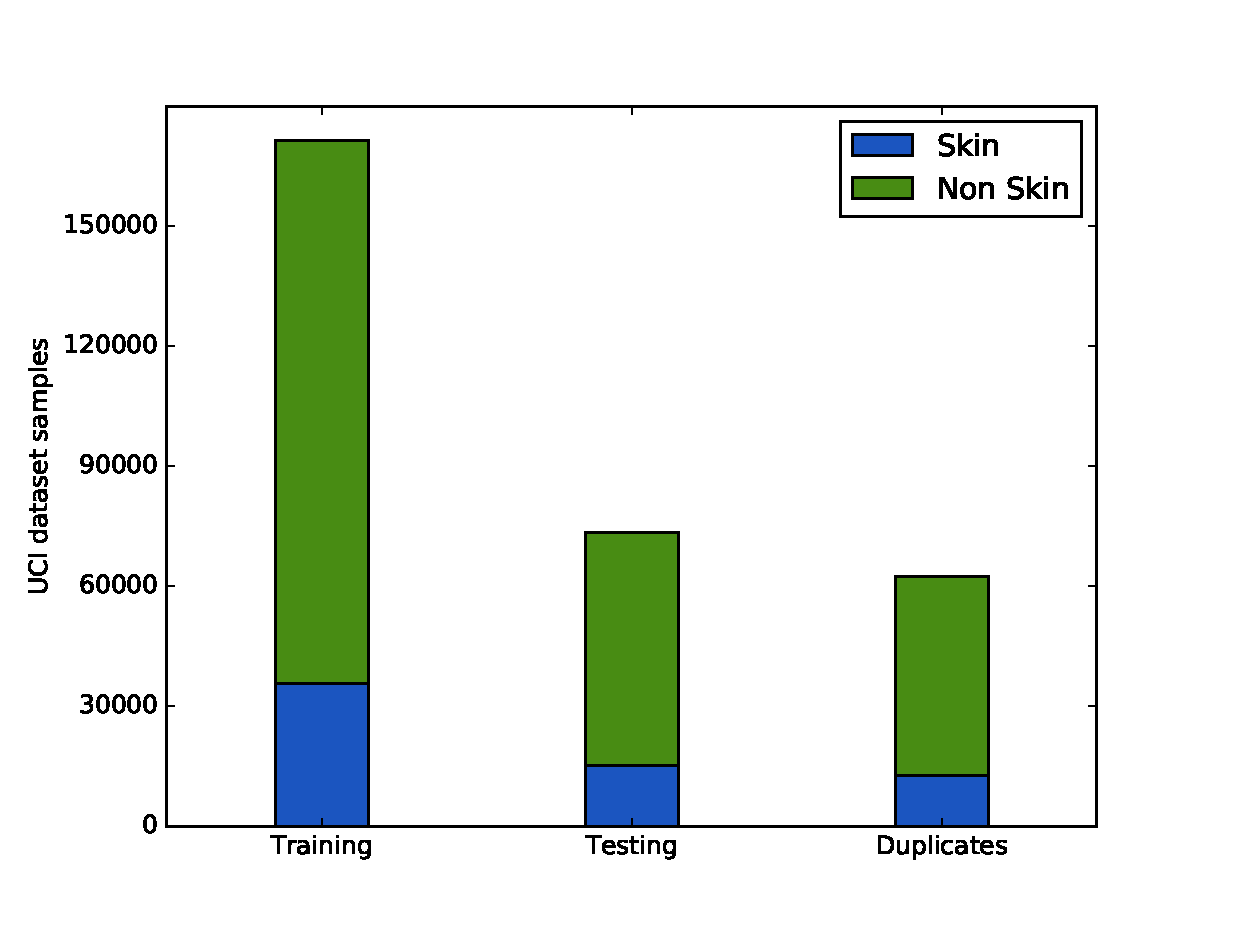
\includegraphics[width=0.85\textwidth]{figuras/uci_split_representation}

    \caption[UCI samples distribution after splitting the dataset in training and testing subsets]{UCI samples distribution after splitting the dataset in training and testing subsets. We used the scikit-learn package function for splitting, where 30\% is the size of test set. The right-most bar, entitled as duplicates, shows how many samples of the test set were seen in training set. In the order of 83\% for skin samples and 86\% for non skin samples. Source: proposed by the author.}
    \label{fig:uci_split_representation}
\end{figure}

For the benefit of the doubt, we submitted the learned function given by those classifiers in real images of Pratheepan and SFA datasets. This experiment can help us to understand the ability of the learned model to generalize for upcoming non seen samples.

\begin{table}[!htpb]
\centering
\begin{small}
\setlength{\tabcolsep}{8pt}

\begin{tabular}{|c|c|c|c|c|c|}\hline
 \thb{Dataset} & \thb{Classifier} & \thb{Precision} & \thbi{Recall} & \thbi{Specificity} & \thbi{F-measure} \\ \hline
 \multirow{2}{*}{SFA} & $k$-NN & 0.9322 & 0.5895 & 0.9835 & 0.7223 \\ \cline{2-6}
                      & SVM    & 0.9079 & 0.4839 & 0.9838 & 0.6314 \\ \hline
 \multirow{2}{*}{Pratheepan} & $k$-NN & 0.5930 & 0.7719 & 0.8568 & 0.6707 \\ \cline{2-6}
                             & SVM    & 0.6179 & 0.7259 & 0.8841 & 0.6675 \\ \hline
\end{tabular}
\end{small}
\caption[Results of the experiments with $k$-NN and SVM in the SFA and Pratheepan images datasets]{Results of the experiments with $k$-NN and SVM in the SFA and Pratheepan images datasets. Despite some of the measures are quite good, we can see that they are far way from the ones given during the training in Table~\ref{tab:results_experiment_one}, which says that the learned models do not have a good generalization.}
\label{tab:results_experiment_one_imgs}
\end{table}

%------------------------------------------------------
\section{Rule-based experiments}
\label{sec:rule_based_experiments}
\noindent In this section we present some experimental evaluations of the proposed extensions described in sections~\ref{sec:proposed_method} and \ref{sec:neighborhood_extended_method}, as well as the original method in  four widely known datasets: SFA, Pratheepan, HGR and Compaq. The latest three of them have also been used in~\citet{brancati:17}.

Table~\ref{tab:merged_rules_results} shows quantitative result metrics of the experiments. Column 1 refers to the dataset used. Column 2 refers to the method being experimented: Original for the original hypothesis;  Reverse refers to the reverse hypothesis with respect to $P_{Cr_{s}}$ parameter; Combined refers to the combination of both of the former methods (see  Sec. \ref{sec:proposed_method}); Neighbors refers to the extension of the method using the neighborhood approach (see  Sec. \ref{sec:neighborhood_extended_method}).


\begin{table*}[ht]
\centering

\begin{tabular}{|c|c|c|c|c|c|c|}\hline
\thb{Dataset} & \thb{Hypothesis} & \thb{Precision} & \thb{Recall} & \thb{Specificity} & \thb{F-measure}\\ \cline{1-6}
\multirow{3}{*}{Compaq}
& Original     & 0.4354            & \textbf{0.8046}   & 0.8046            & 0.5650 \\ \cline{2-6}
& Reverse      & 0.3971            & 0.7232            & 0.7921            & 0.5127 \\ \cline{2-6}
& Combined     & \textbf{0.4906}   & 0.6251            & \textbf{0.8856}   & 0.5498 \\ \cline{2-6}
& Neighbors    & 0.4708            & 0.7421            & 0.8463            & \textbf{0.5761} \\ \hhline{======}

\multirow{3}{*}{Pratheepan}
& Original     & 0.5513            & \textbf{0.8199}   & 0.8230            & 0.6592 \\ \cline{2-6}
& Reverse      & 0.5249            & 0.7326            & 0.8188            & 0.6116 \\ \cline{2-6}
& Combined     & \textbf{0.6681}   & 0.6683            & \textbf{0.9164}   & 0.6682 \\ \cline{2-6}
& Neighbors    & 0.6280            & 0.7515            & 0.8871            & \textbf{0.6843} \\ \hhline{======}

\multirow{3}{*}{HGR}
& Original     & 0.8938            & 0.7664            & 0.9274            & 0.8252 \\ \cline{2-6}
& Reverse      & 0.7929            & \textbf{0.8429}   & 0.8337            & 0.8171 \\ \cline{2-6}
& Combined     & \textbf{0.8994}   & 0.6952            & \textbf{0.9390}   & 0.7843 \\ \cline{2-6}
& Neighbors    & 0.8818            & 0.7935            & 0.9211            & \textbf{0.8353} \\ \hhline{======}

\multirow{3}{*}{SFA}
& Original     & 0.8636             & 0.4214            & 0.9692            & 0.5664 \\ \cline{2-6}
& Reverse      & 0.8563             & \textbf{0.7730}   & 0.9381            & \textbf{0.8125} \\ \cline{2-6}
& Combined     & \textbf{0.9288}    & 0.3958            & \textbf{0.9894}   & 0.5551 \\ \cline{2-6}
& Neighbors    & 0.9176             & 0.5111            & 0.9826            & 0.6565 \\ \hline
\end{tabular}

\caption[Quantitative result metrics of the proposed enhancements and original method]{Quantitative result metrics of the proposed enhancements and \citet{brancati:17}. For each dataset, we have four different applications: the original hypothesis with respect to $P_{Cb_{s}}$, the reverse hypothesis with respect to $P_{Cr_{s}}$, the one which combines both, and the extension using the neighborhood approach.}
\label{tab:merged_rules_results}

\end{table*}

The original method was compared with six well known rule-based methods in literature using four different datasets, three of them, HGR, Pratheepan and Compaq, we have also been used here. We applied the methods against a fourth dataset (SFA) to increase and strengthen the different number of samples tested.

Because the method had the best \textit{F-measure} in the HGR and Pratheepan datasets in comparison with the other six methods and, in addition, because it performed the top first \textit{Precision} in HGR and  second in Pratheepan, we decided to compare the proposed extensions only to the original method.

As one can see in Table~\ref{tab:merged_rules_results}, the reverse hypothesis performed better than the original method and achieved the best \textit{Recall} in HGR and SFA. It also achieved the best \textit{F-measure} in SFA with a 0.8125 rate, which gave almost 0.25 in gain compared to the original.

It is important to note that, the significant improvement of the \textit{Recall} in HGR and SFA datasets is, probably, due to the nature of the images that form each of them. HGR and SFA contain images where we have a great concentration of skin pixels -- hands and arms in the case of HGR, and faces in the case of SFA occupying a considerable region of the image. Furthermore, a large part of them were collected in controlled environments, on the background and lighting conditions point of view. Thus, this behavior must be taken into consideration when selecting the method to apply within an application, since this can be decisive for a potentially performance improvement.

In general, the reverse method increased the \textit{Recall} but did not perform well in \textit{Precision} and \textit{Specificity} measures. When we combined both methods, the best \textit{Precision} and \textit{Specificity} were achieved for all datasets but it loses some performance in \textit{Recall}. However, it still has very good \textit{F-measure} rates.

The neighborhood approach achieved the best \textit{F-measure} in Compaq, HGR, and Pratheepan. Moreover, the other metrics still are in a very high rate for all datasets, being in the top second in almost all cases. If we compare the neighbors approach with the original, except for the \textit{Recall} -- where we only got the best result in SFA --, we can see that our implementation achieved the best measures practically for all other metrics, in the four datasets.

Therefore, the combined and neighbors approaches are very competitive compared to the original method. Furthermore, all the variations of the original method are still computed in quadratic time, maintaining the desired computational efficiency that are useful in different application domains, mainly near real time systems (processing time of about 10ms for a typical image of dimensions 300x400).

Figures~\ref{fig:results_sfa},~\ref{fig:results_pratheepan},~\ref{fig:results_hgr} and~\ref{fig:results_cpq}, present some qualitative results with image samples in column (a) along with the results for each method tested. Column (b) presents the respective ground truth for each image in column (a), column (c) presents the original method~\cite{brancati:17} results, column (d) presents the respective reverse method results, column (e), the combined method results and column (f) the extended neighborhood method.

Qualitatively, we can see that, in general, the reverse method removes a large part of the reddish pixels from the background of the image (e.g. see the third image in the Figure~\ref{fig:results_sfa}, first and fourth images in the Figure~\ref{fig:results_pratheepan}, second image in Figure~\ref{fig:results_hgr}, and third image in Figure~\ref{fig:results_cpq}), which the original method was not able to. On the other hand, the reverse method has not been successful in taking off yellowish-toned background regions (e.g. see the third image in Figure~\ref{fig:results_hgr}, and fifth image in Figure~\ref{fig:results_cpq}).

\begin{figure*}[!htb]
    \centering
    \begin{subfigure}[t]{0.15\textwidth}
        \includegraphics[width=\textwidth]{sfa/ori/img4}
        \includegraphics[width=\textwidth]{sfa/ori/img51}
        \includegraphics[width=\textwidth]{sfa/ori/img112}
        \includegraphics[width=\textwidth]{sfa/ori/img14}
        \caption{}
    \end{subfigure}
    \begin{subfigure}[t]{0.15\textwidth}
        \includegraphics[width=\textwidth]{sfa/gt/img4}
        \includegraphics[width=\textwidth]{sfa/gt/img51}
        \includegraphics[width=\textwidth]{sfa/gt/img112}
        \includegraphics[width=\textwidth]{sfa/gt/img14}
        \caption{}
    \end{subfigure}
    \begin{subfigure}[t]{0.15\textwidth}
        \includegraphics[width=\textwidth]{sfa/cbs/img4}
        \includegraphics[width=\textwidth]{sfa/cbs/img51}
        \includegraphics[width=\textwidth]{sfa/cbs/img112}
        \includegraphics[width=\textwidth]{sfa/cbs/img14}
        \caption{}
    \end{subfigure}
    \begin{subfigure}[t]{0.15\textwidth}
        \includegraphics[width=\textwidth]{sfa/crs/img4}
        \includegraphics[width=\textwidth]{sfa/crs/img51}
        \includegraphics[width=\textwidth]{sfa/crs/img112}
        \includegraphics[width=\textwidth]{sfa/crs/img14}
        \caption{}
    \end{subfigure}
    \begin{subfigure}[t]{0.15\textwidth}
        \includegraphics[width=\textwidth]{sfa/cmb/img4}
        \includegraphics[width=\textwidth]{sfa/cmb/img51}
        \includegraphics[width=\textwidth]{sfa/cmb/img112}
        \includegraphics[width=\textwidth]{sfa/cmb/img14}
        \caption{}
    \end{subfigure}
    \begin{subfigure}[t]{0.15\textwidth}
        \includegraphics[width=\textwidth]{sfa/ngh/img4}
        \includegraphics[width=\textwidth]{sfa/ngh/img51}
        \includegraphics[width=\textwidth]{sfa/ngh/img112}
        \includegraphics[width=\textwidth]{sfa/ngh/img14}
        \caption{}
    \end{subfigure}

    \caption[Image samples with the results of each method in SFA dataset]{Image samples with the results of each method in SFA dataset: (a) original image (b) ground truth (c) original method \cite{brancati:17} (d) reverse method (e) combined method (f) neighbors method.}
    \label{fig:results_sfa}
\end{figure*}

However, when we blend the original method along with the reverse in the method we call combined, both background regions of reddish and yellowish pixels are almost completely removed. In addition, salt-like noises are also dropped, since the rules together are more rigid (e.g. see column (e) combined method for the third image in Figure~\ref{fig:results_hgr}, and fifth image in Figure~\ref{fig:results_cpq}). Obviously, this causes an undesired effect of removing some of the skin pixels of which we are interested. This helps us understand why the recall decreases with the application of the combined rule.

\begin{figure*}[!htb]
    \centering
    \begin{subfigure}[t]{0.15\textwidth}
        \includegraphics[width=2.28cm]{pra/ori/07-c140-12family-red-rr-398h}
        \includegraphics[width=2.28cm]{pra/ori/buck_family}
        \includegraphics[width=2.28cm]{pra/ori/3115267-My-very-large-Indian-family-2}
        \includegraphics[width=2.28cm]{pra/ori/chenhao0017me9}
        \caption{}
    \end{subfigure}
    \begin{subfigure}[t]{0.15\textwidth}
        \includegraphics[width=2.28cm]{pra/gt/07-c140-12family-red-rr-398h}
        \includegraphics[width=2.28cm]{pra/gt/buck_family}
        \includegraphics[width=2.28cm]{pra/gt/3115267-My-very-large-Indian-family-2}
        \includegraphics[width=2.28cm]{pra/gt/chenhao0017me9}
        \caption{}
    \end{subfigure}
    \begin{subfigure}[t]{0.15\textwidth}
        \includegraphics[width=2.28cm]{pra/cbs/07-c140-12family-red-rr-398h}
        \includegraphics[width=2.28cm]{pra/cbs/buck_family}
        \includegraphics[width=2.28cm]{pra/cbs/3115267-My-very-large-Indian-family-2}
        \includegraphics[width=2.28cm]{pra/cbs/chenhao0017me9}
        \caption{}
    \end{subfigure}
    \begin{subfigure}[t]{0.15\textwidth}
        \includegraphics[width=2.28cm]{pra/crs/07-c140-12family-red-rr-398h}
        \includegraphics[width=2.28cm]{pra/crs/buck_family}
        \includegraphics[width=2.28cm]{pra/crs/3115267-My-very-large-Indian-family-2}
        \includegraphics[width=2.28cm]{pra/crs/chenhao0017me9}
        \caption{}
    \end{subfigure}
    \begin{subfigure}[t]{0.15\textwidth}
        \includegraphics[width=2.28cm]{pra/cmb/07-c140-12family-red-rr-398h}
        \includegraphics[width=2.28cm]{pra/cmb/buck_family}
        \includegraphics[width=2.28cm]{pra/cmb/3115267-My-very-large-Indian-family-2}
        \includegraphics[width=2.28cm]{pra/cmb/chenhao0017me9}
        \caption{}
    \end{subfigure}
    \begin{subfigure}[t]{0.15\textwidth}
        \includegraphics[width=2.28cm]{pra/ngh/07-c140-12family-red-rr-398h}
        \includegraphics[width=2.28cm]{pra/ngh/buck_family}
        \includegraphics[width=2.28cm]{pra/ngh/3115267-My-very-large-Indian-family-2}
        \includegraphics[width=2.28cm]{pra/ngh/chenhao0017me9}
        \caption{}
    \end{subfigure}

    \caption[Image samples with the results of each method in Pratheepan dataset]{Image samples with the results of each method in Pratheepan dataset: (a) original image (b) ground truth (c) original method \cite{brancati:17} (d) reverse method (e) combined method (f) neighbors method.}
    \label{fig:results_pratheepan}
\end{figure*}

\begin{figure*}[!htb]
    \centering
    \begin{subfigure}[t]{0.15\textwidth}
        \includegraphics[width=2.28cm]{hgr/ori/D_P_hgr1_id05_2}
        \includegraphics[width=2.28cm]{hgr/ori/N_P_hgr1_id04_5}
        \includegraphics[width=2.28cm]{hgr/ori/V_S_hgr2A2_id03_1}
        \caption{}
    \end{subfigure}
    \begin{subfigure}[t]{0.15\textwidth}
        \includegraphics[width=2.28cm]{hgr/gt/D_P_hgr1_id05_2}
        \includegraphics[width=2.28cm]{hgr/gt/N_P_hgr1_id04_5}
        \includegraphics[width=2.28cm]{hgr/gt/V_S_hgr2A2_id03_1}
        \caption{}
    \end{subfigure}
    \begin{subfigure}[t]{0.15\textwidth}
        \includegraphics[width=2.28cm]{hgr/cbs/D_P_hgr1_id05_2}
        \includegraphics[width=2.28cm]{hgr/cbs/N_P_hgr1_id04_5}
        \includegraphics[width=2.28cm]{hgr/cbs/V_S_hgr2A2_id03_1}
        \caption{}
    \end{subfigure}
    \begin{subfigure}[t]{0.15\textwidth}
        \includegraphics[width=2.28cm]{hgr/crs/D_P_hgr1_id05_2}
        \includegraphics[width=2.28cm]{hgr/crs/N_P_hgr1_id04_5}
        \includegraphics[width=2.28cm]{hgr/crs/V_S_hgr2A2_id03_1}
        \caption{}
    \end{subfigure}
    \begin{subfigure}[t]{0.15\textwidth}
        \includegraphics[width=2.28cm]{hgr/cmb/D_P_hgr1_id05_2}
        \includegraphics[width=2.28cm]{hgr/cmb/N_P_hgr1_id04_5}
        \includegraphics[width=2.28cm]{hgr/cmb/V_S_hgr2A2_id03_1}
        \caption{}
    \end{subfigure}
    \begin{subfigure}[t]{0.15\textwidth}
        \includegraphics[width=2.28cm]{hgr/ngh/D_P_hgr1_id05_2}
        \includegraphics[width=2.28cm]{hgr/ngh/N_P_hgr1_id04_5}
        \includegraphics[width=2.28cm]{hgr/ngh/V_S_hgr2A2_id03_1}
        \caption{}
    \end{subfigure}

    \caption[Image samples with the results of each method in HGR dataset]{Image samples with the results of each method in HGR dataset: (a) original image (b) ground truth (c) original method \cite{brancati:17} (d) reverse method (e) combined method (f) neighbors method.}
    \label{fig:results_hgr}
\end{figure*}

\begin{figure*}[!htb]
    \centering
    \begin{subfigure}[t]{0.15\textwidth}
        \includegraphics[width=\textwidth]{cpq/ori/318196}
        \includegraphics[width=\textwidth]{cpq/ori/795505}
        \includegraphics[width=\textwidth]{cpq/ori/1923132}
        \includegraphics[width=\textwidth]{cpq/ori/2747136}
        \includegraphics[width=\textwidth]{cpq/ori/3003632}
        \caption{}
    \end{subfigure}
    \begin{subfigure}[t]{0.15\textwidth}
        \includegraphics[width=\textwidth]{cpq/gt/318196}
        \includegraphics[width=\textwidth]{cpq/gt/795505}
        \includegraphics[width=\textwidth]{cpq/gt/1923132}
        \includegraphics[width=\textwidth]{cpq/gt/2747136}
        \includegraphics[width=\textwidth]{cpq/gt/3003632}
        \caption{}
    \end{subfigure}
    \begin{subfigure}[t]{0.15\textwidth}
        \includegraphics[width=\textwidth]{cpq/cbs/318196}
        \includegraphics[width=\textwidth]{cpq/cbs/795505}
        \includegraphics[width=\textwidth]{cpq/cbs/1923132}
        \includegraphics[width=\textwidth]{cpq/cbs/2747136}
        \includegraphics[width=\textwidth]{cpq/cbs/3003632}
        \caption{}
    \end{subfigure}
    \begin{subfigure}[t]{0.15\textwidth}
        \includegraphics[width=\textwidth]{cpq/crs/318196}
        \includegraphics[width=\textwidth]{cpq/crs/795505}
        \includegraphics[width=\textwidth]{cpq/crs/1923132}
        \includegraphics[width=\textwidth]{cpq/crs/2747136}
        \includegraphics[width=\textwidth]{cpq/crs/3003632}
        \caption{}
    \end{subfigure}
    \begin{subfigure}[t]{0.15\textwidth}
        \includegraphics[width=\textwidth]{cpq/cmb/318196}
        \includegraphics[width=\textwidth]{cpq/cmb/795505}
        \includegraphics[width=\textwidth]{cpq/cmb/1923132}
        \includegraphics[width=\textwidth]{cpq/cmb/2747136}
        \includegraphics[width=\textwidth]{cpq/cmb/3003632}
        \caption{}
    \end{subfigure}
    \begin{subfigure}[t]{0.15\textwidth}
        \includegraphics[width=\textwidth]{cpq/ngh/318196}
        \includegraphics[width=\textwidth]{cpq/ngh/795505}
        \includegraphics[width=\textwidth]{cpq/ngh/1923132}
        \includegraphics[width=\textwidth]{cpq/ngh/2747136}
        \includegraphics[width=\textwidth]{cpq/ngh/3003632}
        \caption{}
    \end{subfigure}

    \caption[Image samples with the results of each method in Compaq dataset]{Image samples with the results of each method in Compaq dataset: (a) original image (b) ground truth (c) original method \cite{brancati:17} (d) reverse method (e) combined method (f) neighbors method.}
    \label{fig:results_cpq}
\end{figure*}
\clearpage

%% ------------------------------------------------------------------------- %%
\section{Supplementary neighborhood operations experiments}
\label{sec:sno_experiments}
In this section we will show some experimental results of the supplementary neighborhood adaptation described in section~\ref{sec:sup_neighborhood_operations}. In short, we basically scan the image, with a size of $W \times H$, in the raster order, and apply the original and reverse rules for every single pixel. We keep the result in a matrix of the same size ($W \times H$) of the input image. For each coordinate of this output matrix, we will have a two positions vector with the result of the original and reverse rules answer for this pixel. Finally, we count those answers in four different strategies. The results can be seen in table~\ref{tab:sup_neighbors_results}.

\begin{table*}[ht]
\centering

\begin{tabular}{|c|c|c|c|c|c|c|}\hline
\thb{Dataset} & \thb{\vtop{\hbox{\strut Hypothesis}\hbox{\strut (Neighbors)}}} & \thb{Precision} & \thb{Recall} & \thb{Specificity} & \thb{F-measure}\\ \cline{1-6}
\multirow{3}{*}{Compaq}
& AND               & \textbf{0.5121}   & 0.6252            & \textbf{0.8941}   & 0.5630 \\ \cline{2-6}
& OR                & 0.3786            & \textbf{0.9037}   & 0.7203            & 0.5336 \\ \cline{2-6}
& $P_{Cr_s}$ only   & 0.4132            & 0.7254            & 0.8032            & 0.5265 \\ \cline{2-6}
& $P_{Cb_s}$ only   & 0.4478            & 0.8053            & 0.8120            & \textbf{0.5755} \\ \hhline{======}

\multirow{3}{*}{Pratheepan}
& AND               & \textbf{0.6731}   & 0.6789            & \textbf{0.9127}   & \textbf{0.6760} \\ \cline{2-6}
& OR                & 0.4624            & \textbf{0.8837}   & 0.7321            & 0.6072 \\ \cline{2-6}
& $P_{Cr_s}$ only   & 0.5285            & 0.7414            & 0.8163            & 0.6171 \\ \cline{2-6}
& $P_{Cb_s}$ only   & 0.5630            & 0.8218            & 0.8292            & 0.6682 \\ \hhline{======}

\multirow{3}{*}{HGR}
& AND               & \textbf{0.9007}   & 0.7203            & \textbf{0.9378}   & 0.8005 \\ \cline{2-6}
& OR                & 0.7978            & \textbf{0.9084}   & 0.8238            & \textbf{0.8495} \\ \cline{2-6}
& $P_{Cr_s}$ only   & 0.7937            & 0.8600            & 0.8331            & 0.8256 \\ \cline{2-6}
& $P_{Cb_s}$ only   & 0.8818            & 0.7935            & 0.9211            & 0.8353 \\ \hhline{======}

\multirow{3}{*}{SFA}
& AND               & \textbf{0.9345}   & 0.3947            & \textbf{0.9899}   & 0.5549 \\ \cline{2-6}
& OR                & 0.8345            & \textbf{0.8181}   & 0.9176            & 0.8262 \\ \cline{2-6}
& $P_{Cr_s}$ only   & 0.8612            & 0.7922            & 0.9375            & 0.8252 \\ \cline{2-6}
& $P_{Cb_s}$ only   & 0.8953            & 0.7690            & 0.9286            & \textbf{0.8273} \\ \hline
\end{tabular}

\caption[Quantitative result metrics of the proposed supplementary neighborhood adaptation]{Quantitative result metrics of the proposed supplementary neighborhood adaptation. For each dataset, we have four different applications of the neighbors operations, respectively: applying an AND between the original and reverse rules, applying an OR between the original and reverse rules, considering the $P_{Cr_{s}}$ (reverse) only, and considering the $P_{Cb_{s}}$ (original) only.}
\label{tab:sup_neighbors_results}

\end{table*}

It is worth mentioning that the goal here is to explore better the connectivity of the 8-\textit{neighbors} window and check, on the basis of a symmetric mask window, if the \textit{diagonal effect} is gone as well as the measures are improved. Therefore, we are not worried about the additional computational cost taken to scan the image one more time. Even though, this implementation can be enhanced by, for instance, keeping the latest three lines of the image scanned in memory to be verified by the 8-\textit{neighbors} window backward to have a final decision when evaluating a pixel.

From the table~\ref{tab:sup_neighbors_results} we can see that the application of the neighborhood approach using AND gives us the best precision and specificity in all datasets. On the other hand, we lost performance in the recall in relation to the others approaches. Speaking of recall, the loss is in the order of 20\% up to 30\% in the Compaq, Pratheepan and HGR datasets, and approximately 50\% in the SFA.

Clearly there is a trade-off between increasing precision and decreasing recall and vice versa, just as in the experiments done in section~\ref{sec:rule_based_experiments} with all methods. When we use a more relaxed rule, as in the case of the OR or the isolated rules, we get a better recall, but there is also an abrupt drop in precision and specificity. Another side effect of this phenomenon is to increase the false positive rate.

The AND conjunction approach is most similar to that implemented in neighborhood extended method (see Sec.~\ref{sec:neighborhood_extended_method}). The results obtained by that approach show low variability in relation to the adaptations shown in the experiments in this section. Therefore, for the sake of implementation, the approach given in the neighborhood implementation may be a good starting point. Nevertheless, we can apply some other complementary technique, such as weights in the pixels, to measure those more or less relevant to the decision making in the neighborhood. This can potentially diminish the effect of this trade-off and obtain more harmonic measures while removing the undesired \textit{diagonal effect}.


%------------------------------------------------------
\section{Grid search parameters experiments}
\label{sec:grid_search_experiments}
In one part of this work we are concerned with understanding and, perhaps, improving the choice of parameters that define the trapezoids. They are a fundamental part of the model that segments the skin pixels in an image, the main role of the methods developed here. In short, as described in section~\ref{sec:trapezoids_params_tunning}, 5${th}$ and 95$th$ percentiles of the histogram of $Y$ luminance component have been used by~\citet{brancati:17} to be the right parameters to define the trapezoids coordinates. For this reason, we decided to shot different combination of these parameters to figure out which pair better works for the model fitting. In addition, we would like to answer the question: why 5${th}$ and 95$th$ percentiles have been used?

Thus, we created a simple grid search algorithm (see details in section~\ref{sec:trapezoids_params_tunning}) to find the best range combination of those parameters. Despite we do not exhaustively consider all parameter combinations, we used an efficient search strategy by sampling a given number of candidates. For each chosen parameters candidate, we dynamically used them in the combined method to test every single image of each dataset described in section~\ref{sec:datasets}. Lastly, we sort the results table using respectively, \emph{F-measure}, \emph{Precision}, and \emph{Recall} metrics. The results with these metrics, in that given order, for each dataset, can be seen in Appendix~\ref{ape:trapezoids_parameters_tuning}.

It is worth mentioning that the grid search algorithm starts with $P_{min}$ percentile index in $5$ and $P_{max}$ percentile lower bound is set to $P_{min}$ in the inner loop. Thus, we will no longer have a combination of parameters such as $[15, 10]$, that means, we always have combinations such that $P_{max} \geq P_{min}$. This will produce a table with results according the template given in Figure~\ref{fig:gs_table_output}.

\begin{figure}[ht]
    \centering
    \begin{tikzpicture}
    \draw[step=0.75cm,black,thin] (0.75,0.75) grid (4.5,4.5);

    %gray area
    \foreach \k in {0.75,1.5,...,3.75}{
        \fill[pattern=north east lines, pattern color=gray] (\k,3.75) rectangle (\k+0.75,4.5);
    }
    \foreach \k in {1.5,2.25,...,3.75}{
        \fill[pattern=north east lines, pattern color=gray] (\k,3) rectangle (\k+0.75,3.75);
    }
    \foreach \k in {2.25,3,...,3.75}{
        \fill[pattern=north east lines, pattern color=gray] (\k,2.25) rectangle (\k+0.75,3);
    }
    \fill[pattern=north east lines, pattern color=gray] (3,1.5) rectangle (3.75,2.25);
    \fill[pattern=north east lines, pattern color=gray] (3.75,1.5) rectangle (4.5,2.25);
    \fill[pattern=north east lines, pattern color=gray] (3.75,0.75) rectangle (4.5,1.5);

    % labels outside
    \node at (0.375,1.125) {95};
    \node at (0.375,1.875) {90};
    \node at (0.375,2.625) {\vdots};
    \node at (0.375,3.375) {10};
    \node at (0.375,4.125) {5};
    \node at (1.125,4.875) {5};
    \node at (1.875,4.875) {10};
    \node at (2.625,4.875) {\ldots};
    \node at (3.375,4.875) {90};
    \node at (4.125,4.875) {95};
    \end{tikzpicture}

    \caption[The output template table with result metrics of the grid search algorithm]{The output template table with result metrics of the grid search algorithm. $P_{min}$ percentile index is in vertical axis and $P_{max}$ percentile index is in horizontal axis. The highlighted cells -- from the main diagonal and above -- are the ones which will have values of the metrics after running the method for the given combination of parameters. Source: proposed by the author.}
    \label{fig:gs_table_output}
\end{figure}

We performed this experiment in all four datasets: Compaq, Pratheepan, HGR, and SFA. For each dataset, respectively, we have a scatter plot of \emph{F-measure}, \emph{Precision}, and \emph{Recall}, which can be seen in Figures~\ref{fig:compaq_g_search},~\ref{fig:pratheepan_g_search},~\ref{fig:hgr_g_search}, and~\ref{fig:sfa_g_search}\footnote{The scatter plots are ignoring the results when $P_{min} = P_{max}$ since they are always the same.}. Each series is represented by a shade of a gradient color. In other words, the darkest is the color the lower is the $P_{min}$ fixed value while $P_{max}$ is varying along $x$ (horizontal) axis.

In general, the points on the upper-right side of the charts are the ones with the best metric result for each parameters' combination. We can see predominantly that larger intervals -- e.g. $[5, 85]$, $[5, 90]$, $[5, 95]$ -- resulted in the best \emph{Precision}. On the other hand, smaller intervals, with both $P_{min}$ and $P_{max}$ near the upper bound (95) -- e.g. $[80, 90]$, $[85, 95]$, $[90 ,95]$ --, performed better in \emph{Recall}. Thus, if we set up a specific pair of parameters for the percentile to compute the trapezoid coordinates, it can produce a good \emph{Precision} but it may hurt the \emph{Recall} and vice versa.

Therefore, evaluate \emph{F-measure} in this situation seems to be the correct path, since it gives us a harmonic measure between \emph{Precision} and \emph{Recall}. That's why we sorted the results (see Tables~\ref{tab:compaq_grid_search},~\ref{tab:pratheepan_grid_search},~\ref{tab:hgr_grid_search}, and~\ref{tab:sfa_grid_search} for details) using the order \emph{F-measure}, \emph{Precision}, and \emph{Recall} as a criteria.

In Compaq, we can see that top \emph{F-measure} results were obtained with pair of parameters such as $[5, 25], \ldots, [5, 95]$, while keeping good measures in both \emph{Precision} and \emph{Recall}. A similar behavior can be seen in Pratheepan, but among the highest \emph{F-measure} scores are those where $P_{min} = 10$ -- i.e. $[10, 25], \ldots, [10, 95]$. Next in sequence are those starting with $P_{min} = 5$. So, we could state that the values $[5, 95]$ chosen by~\citet{brancati:17} are fair enough since the results were quite good. Even so, the results are insignificantly worse than the highest ranked ones (see Table~\ref{tab:gs_results_comparison}).

However, in HGR as well as in SFA top \emph{F-measure} results were obtained with pair of parameters such that $P_{min} = P_{max}$. For instance, we can see in HGR results that \emph{Recall} = 0.8623 and \emph{F-measure} = 0.8664 when $P_{min} = 5$ and $P_{max} = 5$, while $[5, 95]$ interval resulted in \emph{Recall} = 0.6952 and \emph{F-measure} = 0.7843 -- a gain in the order of 24\% and 10\% for each metric, respectively. A similar behavior can be seen in the results of SFA, where the gain in \emph{Recall} and \emph{F-measure} are in the order of 65\% and 38\% for each metric, respectively, which is a very huge difference.



\begin{table*}[ht]
\centering

\begin{tabular}{|c|c|c|c|c|c|c|c|}\hline
\thb{Dataset} & \textbf{$P_{min}$} & \textbf{$P_{max}$} & \thb{Precision} & \thb{Recall} & \thb{Specificity} & \thb{F-measure}\\ \cline{1-7}
\multirow{3}{*}{Compaq}
& 5  &   95  & 0.4906    &   0.6251  &   0.8856  & 0.5498 \\ \cline{2-7}
& 5  &   25  & 0.4896    &   0.6334  &   0.8826  & 0.5523 \\ \cline{2-7}
& 5  &   20  & 0.4862    &   0.6387  &   0.8794  & 0.5521 \\ \cline{2-7}
& 5  &   35  & 0.4939    &   0.6249  &   0.8870  & 0.5517 \\ \hhline{=======}

\multirow{3}{*}{Pratheepan}
& 5  &   95  & 0.6681    &   0.6683  &   0.9164  & 0.6682 \\ \cline{2-7}
& 10 &   15  & 0.6531    &   0.7001  &   0.9066  & 0.6758 \\ \cline{2-7}
& 5  &   15  & 0.6639    &   0.6857  &   0.9133  & 0.6746 \\ \cline{2-7}
& 10 &   55  & 0.6660    &   0.6829  &   0.9137  & 0.6744 \\ \hhline{=======}

\multirow{3}{*}{HGR}
& 5  &   95  & 0.8994    &   0.6952  &   0.9390  & 0.7843 \\ \cline{2-7}
& 5  &   5   & 0.8706    &   0.8623  &   0.9073  & 0.8664 \\ \cline{2-7}
& 10 &   10  & 0.8706    &   0.8623  &   0.9073  & 0.8664 \\ \cline{2-7}
& 15 &   15  & 0.8706    &   0.8623  &   0.9073  & 0.8664 \\ \hhline{=======}

\multirow{3}{*}{SFA}
& 5  &   95  & 0.9288    &   0.3958  &   0.9894  & 0.5551 \\ \cline{2-7}
& 5  &   5   & 0.9319    &   0.6567  &   0.9789  & 0.7705 \\ \cline{2-7}
& 10 &   10  & 0.9319    &   0.6567  &   0.9789  & 0.7705 \\ \cline{2-7}
& 15 &   15  & 0.9319    &   0.6567  &   0.9789  & 0.7705 \\ \hline
\end{tabular}

\caption[Quantitative result metrics of the proposed grid search parameters tuning]{Quantitative result metrics of the proposed grid search parameters tuning. For each dataset, we have four different applications of the combined method with different pairs of $P_{min}$ and $P_{max}$ percentiles. The first line is the default one $[5, 95]$, as reported in the experiments given in Table~\ref{tab:results_experiment_one}. Next three lines are the top three results ordered by F-measure, Precision, and Recall, respectively.}
\label{tab:gs_results_comparison}

\end{table*}


On the basis of this scenario, we observed that when we have $P_{min} = P_{max}$, the resulting metric is absolute the same for any combination of equal percentile parameters. For instance, in Compaq dataset, when we tried $P_{min} = 5$ and $P_{max} = 5$, we got \emph{Precision} = 0.4180, \emph{Recall} = 0.7323, \emph{Specificity} = 0.8105, and \emph{F-measure} = 0.5322. The result is the same for $P_{min} = 10$ and $P_{max} = 10$ onward up to $P_{min} = 95$ and $P_{max} = 95$. This behavior will repeat for every single dataset tested.

Based on this result, we started to investigate the source code given in the original method by~\citet{brancati:17}. We found out that, when the percentiles are the same, the computation of the parameters who define the trapezoids is impacted. In other words, $Y_0$, $Y_1$, $Y_2$, $Y_3$, $Y_{min}$, $Y_{max}$, $Cr_{min}$, $Cb_{max}$ are always the same, i.e. assume default values. Even $Cb_{min}$, $Cr_{max}$, that are still computed dynamically by the internal method functions, do not change when $P_{min}$, $P_{max}$ percentiles are changed, since they are dependent on the previous parameters and the histogram of the image itself that never change. The same behavior will be observed when $P_{min} > P_{max}$.

It is important to note that, in the case of Compaq and Pratheepan, where $P_{min} = P_{max}$, the results worsen significantly. On the other hand, they have a significant gain in the HGR and SFA datasets.

This particular phenomenon occurs by the nature of the images that form each of these images databases. Both Compaq and Pratheepan contain images with more complex scenes, uncontrolled environment, distinct lighting conditions and, in general, images randomly collected from the internet. On the other hand, HGR and SFA contain images where we have a great concentration of skin pixels -- hands and arms in the case of HGR, and faces in the case of SFA occupying a considerable region of the image. Furthermore, a large part of them were collected in controlled environments, on the background and lighting conditions point of view.

Therefore, this behavior must be taken into consideration when selecting a pair of $P_{min}$ and $P_{max}$ to apply in the method in question, since this can be decisive for a potentially performance improvement.

\clearpage % to avoid warnings on 'Text page X contains only floats.'
\begin{figure}[!htb]
    \centering
    \begin{subfigure}[t]{0.95\textwidth}
        \includegraphics[width=\textwidth]{g_search/compaq_precision}
    \end{subfigure}
    \begin{subfigure}[t]{0.95\textwidth}
        \includegraphics[width=\textwidth]{g_search/compaq_recall}
    \end{subfigure}
    \begin{subfigure}[t]{0.95\textwidth}
        \includegraphics[width=\textwidth]{g_search/compaq_fmeasure}
    \end{subfigure}
    \caption[Scatter plot with the quality measures for grid search parameters in Compaq dataset]{Scatter plot with the quality measures for grid search parameters in Compaq dataset.In $y$ axis we have the measure for each combination. In $x$ axis we are varying the $y$ maximum percentile. Each series represent a fixed $y$ minimum percentile.}
    \label{fig:compaq_g_search}
\end{figure}


\clearpage % to avoid warnings on 'Text page X contains only floats.'
\begin{figure}[!htb]
    \centering
    \begin{subfigure}[t]{0.95\textwidth}
        \includegraphics[width=\textwidth]{g_search/pratheepan_precision}
    \end{subfigure}
    \begin{subfigure}[t]{0.95\textwidth}
        \includegraphics[width=\textwidth]{g_search/pratheepan_recall}
    \end{subfigure}
    \begin{subfigure}[t]{0.95\textwidth}
        \includegraphics[width=\textwidth]{g_search/pratheepan_fmeasure}
    \end{subfigure}
    \caption[Scatter plot with the quality measures for grid search parameters in Pratheepan dataset]{Scatter plot with the quality measures for grid search parameters in Pratheepan dataset.In $y$ axis we have the measure for each combination. In $x$ axis we are varying the $y$ maximum percentile. Each series represent a fixed $y$ minimum percentile.}
    \label{fig:pratheepan_g_search}
\end{figure}


\clearpage % to avoid warnings on 'Text page X contains only floats.'
\begin{figure}[!htb]
    \centering
    \begin{subfigure}[t]{0.95\textwidth}
        \includegraphics[width=\textwidth]{g_search/hgr_precision}
    \end{subfigure}
    \begin{subfigure}[t]{0.95\textwidth}
        \includegraphics[width=\textwidth]{g_search/hgr_recall}
    \end{subfigure}
    \begin{subfigure}[t]{0.95\textwidth}
        \includegraphics[width=\textwidth]{g_search/hgr_fmeasure}
    \end{subfigure}
    \caption[Scatter plot with the quality measures for grid search parameters in HGR dataset]{Scatter plot with the quality measures for grid search parameters in HGR dataset.In $y$ axis we have the measure for each combination. In $x$ axis we are varying the $y$ maximum percentile. Each series represent a fixed $y$ minimum percentile.}
    \label{fig:hgr_g_search}
\end{figure}


\clearpage % to avoid warnings on 'Text page X contains only floats.'
\begin{figure}[!htb]
    \centering
    \begin{subfigure}[t]{0.95\textwidth}
        \includegraphics[width=\textwidth]{g_search/sfa_precision}
    \end{subfigure}
    \begin{subfigure}[t]{0.95\textwidth}
        \includegraphics[width=\textwidth]{g_search/sfa_recall}
    \end{subfigure}
    \begin{subfigure}[t]{0.95\textwidth}
        \includegraphics[width=\textwidth]{g_search/sfa_fmeasure}
    \end{subfigure}
    \caption[Scatter plot with the quality measures for grid search parameters in SFA dataset]{Scatter plot with the quality measures for grid search parameters in SFA dataset.In $y$ axis we have the measure for each combination. In $x$ axis we are varying the $y$ maximum percentile. Each series represent a fixed $y$ minimum percentile.}
    \label{fig:sfa_g_search}
\end{figure}